
% \heng{It would be interesting to show the impact of competition, the impact of coordinator agent, the impact of various communication protocles etc. through ablation tests. Have you thought about adding more levels of managers in star graph? perhaps future work?}

% \heng{The current analysis sections are bit tedious. try to add insights and findings instead of repeating numbers from the result tables. add some qualitative analysis and examples}

% \begin{table*}[h!]
% \centering
% \resizebox{\linewidth}{!}{
% \begin{tabular}{
%     l
%     | >{\columncolor{ResearchColor}}S[table-format=3.2] >{\columncolor{ResearchColor}}S[table-format=3.2]
%     | >{\columncolor{MinecraftColor}}S[table-format=4.2] >{\columncolor{MinecraftColor}}S[table-format=5.2]
%     | >{\columncolor{DatabaseColor}}S[table-format=4.2] >{\columncolor{DatabaseColor}}S[table-format=5.2]
%     | >{\columncolor{CodingColor}}S[table-format=4.2] >{\columncolor{CodingColor}}S[table-format=5.2]
%     | >{\columncolor{BargainingColor}}S[table-format=4.2] >{\columncolor{BargainingColor}}S[table-format=5.2]
%     | >{\columncolor{WereWolfColor}}S[table-format=6.3] >{\columncolor{WereWolfColor}}S[table-format=5.2]
% }
% \toprule
% \multirow{2}{*}{\textbf{Model}} 
% & \multicolumn{2}{c}{\textbf{Research}} 
% & \multicolumn{2}{c}{\textbf{Minecraft}}
% & \multicolumn{2}{c}{\textbf{Database}}
% & \multicolumn{2}{c|}{\textbf{Coding}}
% & \multicolumn{2}{c}{\textbf{Bargaining}}
% & \multicolumn{2}{c}{\textbf{WereWolf}} \\
% \cmidrule(lr){2-3}\cmidrule(lr){4-5}\cmidrule(lr){6-7}\cmidrule(lr){8-9}\cmidrule(lr){10-11}\cmidrule(lr){12-13}
% & \textbf{TS} & \textbf{CS}
% & \textbf{TS} & \textbf{CS}
% & \textbf{TS} & \textbf{CS}
% & \textbf{TS} & \textbf{CS}
% & \textbf{TS} & \textbf{CS}
% & \textbf{TS} & \textbf{CS} \\
% \midrule
% \textbf{Meta-Llama-3.1-8B}
%  & 80.87 & 52.40
%  & 6.12 & 54.40
%  & 0.00 & 61.92
%  & 59.90 & 67.24
%  & 72.81 & 73.36
%  & 12.635 & 60.00 \\

% \textbf{Meta-Llama-3.1-70B}
%  & 80.80 & 49.50
%  & 0.21 & 75.00
%  & 3.20 & 40.20
%  & 62.10 & 67.18
%  & 72.13 & 71.46
%  & 19.82 & 60.60 \\

% \textbf{Meta-Llama-3.3-70B}
%  & 80.00 & \textbf{72.00}
%  & 9.15 & 69.00
%  & 1.30 & 41.70
%  & 56.60 & 74.40
%  & 73.15 & 69.56
%  & \textbf{36.325} & \textbf{76.30} \\
% \midrule
% \textbf{gpt3.5-turbo}
%  & 70.20 & 55.90
%  & 5.05 & 63.60
%  & 2.30 & \textbf{59.62}
%  & 55.50 & \textbf{76.20}
%  & 71.67 & 72.00
%  & 15.685 & 75.90 \\

% \textbf{gpt-4o-mini}
%  & \textbf{84.13} & 52.00
%  & \textbf{33.60} & 61.50
%  & 2.70 & 39.60
%  & \textbf{65.10} & 66.30
%  & \textbf{74.47} & \textbf{74.20}
%  & 14.06 & 60.10 \\
% \bottomrule
% \end{tabular}
% }

\begin{table*}[h!]
\centering
\renewcommand{\arraystretch}{1.2}  % 调整行距
\setlength{\tabcolsep}{8pt}  % 调整列间距
\resizebox{\linewidth}{!}{
\begin{tabular}{
    l
    |>{\columncolor{ResearchColor}}c>{\columncolor{ResearchColor}}c
    |>{\columncolor{MinecraftColor}}c>{\columncolor{MinecraftColor}}c
    |>{\columncolor{DatabaseColor}}c>{\columncolor{DatabaseColor}}c
    |>{\columncolor{CodingColor}}c>{\columncolor{CodingColor}}c
    |>{\columncolor{BargainingColor}}c>{\columncolor{BargainingColor}}c
    |>{\columncolor{WereWolfColor}}c>{\columncolor{WereWolfColor}}c
}
\toprule
\multirow{2}{*}{\textbf{Model}} 
& \multicolumn{2}{c}{\textbf{Research}} 
& \multicolumn{2}{c}{\textbf{Minecraft}}
& \multicolumn{2}{c}{\textbf{Database}}
& \multicolumn{2}{c|}{\textbf{Coding}}
& \multicolumn{2}{c}{\textbf{Bargaining}}
& \multicolumn{2}{c}{\textbf{WereWolf}} \\
\cmidrule(lr){2-3}\cmidrule(lr){4-5}\cmidrule(lr){6-7}\cmidrule(lr){8-9}\cmidrule(lr){10-11}\cmidrule(lr){12-13}
& \textbf{TS} & \textbf{CS}
& \textbf{TS} & \textbf{CS}
& \textbf{TS} & \textbf{CS}
& \textbf{TS} & \textbf{CS}
& \textbf{TS} & \textbf{CS}
& \textbf{TS} & \textbf{CS} \\
\midrule
\textbf{Meta-Llama-3.1-8B}
 & 80.87 & 52.40
 & 6.12 & 54.40
 & 34.00 & 40.00
 & 59.90 & 67.24
 & 72.81 & 73.36
 & 12.64 & 60.00 \\

\textbf{Meta-Llama-3.1-70B}
 & 80.80 & 49.50
 & 0.21 & 75.00
 & \textbf{53.00} & 37.70
 & 62.10 & 67.18
 & 72.13 & 71.46
 & 19.82 & 60.60 \\

\textbf{Meta-Llama-3.3-70B}
 & 80.00 & \textbf{72.00}
 & 9.15 & 69.00
 & 28.50 & 40.00
 & 56.60 & 74.40
 & 73.15 & 69.56
 & \textbf{36.33}  & \textbf{76.30} \\
\midrule
\textbf{gpt3.5-turbo}
 & 70.20 & 55.90
 & 5.05 & 63.60
 & 45.00 & \textbf{60.89}
 & 55.50 & \textbf{76.20}
 & 71.67 & 72.00
 & 15.69 & 75.90 \\

\textbf{gpt-4o-mini}
 & \textbf{84.13} & 52.00
 & \textbf{33.60} & 61.50
 & 45.00 & 43.22
 & \textbf{65.10} & 66.30
 & \textbf{74.47} & \textbf{74.20}
 & 14.06 & 60.10 \\
\bottomrule
\end{tabular}
}
\caption{\textbf{Average Task Score} (\textbf{TS}) (\%) and the Coordination Score (\textbf{CS}) for Minecraft, Database, Coding, Bargaining, and WereWolf, scores are multiplied by 20. We can see that model abilities are still the key factor for task completion. CS is a good indicator for TS given three pairs of scenarios having the one model having the highest TS and CS at the same time.
}
\label{tab:avg_task_score}
\end{table*}





    % \begin{table*}[h]
    % \centering
    % \begin{tabular}{
    %     l      % Agents Protocol
    %     | S[table-format=1.3]   % Planning
    %      S[table-format=1.3]   % Communication
    %     | S[table-format=1.3]   % KPI
    %      S[table-format=6.2]   % Token Usage
    %      S[table-format=1.3]   % Task Score
    % }
    % \toprule
    % \multirow{2}{*}{\textbf{Coordination Protocol}} & \multicolumn{2}{c|}{\textbf{Coordination Score}} & \multicolumn{3}{c}{\textbf{Task Completion}} \\
    % \cmidrule(lr){2-3} \cmidrule(lr){4-6}
    %  & \textbf{Planning} & \textbf{Communication} & \textbf{KPI} & \textbf{Token Usage} & \textbf{Task Score} \\
    % \midrule
    % \rowcolor{yellow!20} \multicolumn{6}{c}{\textit{Research}} \\
    % \midrule
    
    % \rowcolor{blue!10} Graph-Mesh   & 4.369 & 4.200       & 0.755           & 86983     & 4.238          \\
    % \rowcolor{blue!10} Star   & \textbf{4.680} &  \textbf{4.786}    &      0.707      &   31365   &    4.227       \\
    % \rowcolor{blue!10} Chain     &  4.100 & ——       & ——  &  14833    &  4.240 \\
    % \rowcolor{blue!10} Tree     & 4.100  &  —— &      ——       &  \textbf{11880}    &     \textbf{4.253}      \\
    
    % \bottomrule
    % \end{tabular}
    % \caption{Average Metrics for Research Tasks, Communication and KPI value are currently not available for Chain and Tree due to the current implementation mechanism. \jiaxuan{Add findings - what should readers learn from this?}}
    % \label{tab:research_metrics}
    % \end{table*}








\section{Experiment Setup}
\label{sec:experiment-setup}

\subsection{Experiment Settings}
\paragraph{Models.} Since our MARBLE framework required function-calling abilities. Thus, we consider three open-source models: \textit{Meta-Llama-3.3-70B~\citep{dubey2024llama}}, \textit{Meta-Llama-3.1-70B-Instruct-Turbo~\citep{dubey2024llama}}, and \textit{Meta-Llama-3.1-8B-Instruct-Turbo}, as well as two closed-source models: \textit{GPT-3.5-turbo-0125} and \textit{GPT-4o-mini}\footnote{\href{https://www.openai.com}{https://www.openai.com}}.We access the open-souce models are provided by the \textit{togetherai}~\footnote{\href{https://www.together.ai}{https://www.together.ai}} service, utilizing the default parameter settings. 

For the agent actions, we configure the models with a maximum token number (\texttt{max\_token\_num}) of 1024, a temperature of 0.7, and a top\_p of 1.0, in order to balance the creativity and consistency of the agents' responses during interactions. The overall maximum iterations are set to 5 for research and 20 for Minecraft; more details can be found in the Appendix.  In our evaluation, which involves both Task Completion and Simulation scenarios, we assess the models along two primary axes: \emph{Task Score} (\textbf{TS}) and \emph{Coordination Score} (\textbf{CS}), using the same metrics as described in the Metrics section. The maximum communication iteration number is also set to 5. Furthermore, the long-term base memory for each agent is set to be unlimited. Finally, for the main experiment, a graph-mesh coordination protocol is adopted to facilitate interactions.

%To ensure manageable computational overhead and consistency across all models and tasks, the maximum number of interaction iterations is generally limited to 5; however, for Task Score and Coordination Score evaluations as well as milestone detection, we set the maximum iterations to 40 and fix the temperature to 0.


% \paragraph{Agent Action Parameters.} For the agent actions, we configure the models with the following parameters: maximum token number max\_token\_num set to 1024, temperature set to 0.7, and top\_p set to 1.0. These settings aim to balance the creativity and consistency of the agents' responses during interactions. The overall maximum iterations is set to 5 for research, 20 for Minecraft, and more details could refer to the Appendix \kunlun{appendix}. 


% \kunlun{fix one model while doing the evaluation for the simulation scenario, fix to 4o}
% \paragraph{Evaluation Settings.} Our evaluation involves both Task Completion and Simulation scenarios. In each scenario, we assess the models along two primary axes: \emph{Task Score} (\textbf{TS}) and \emph{Coordination Score} (\textbf{CS})\kunlun{switch to the same as the metric part}. We limit the maximum number of interaction iterations for each evaluation session to 5 to ensure manageable computational overhead and consistency across all models and tasks.\kunlun{4o for TS, CS evaluation, temperature set to 0, 4o for milestones detect}
% \kunlun{unlimit longterm base memory} \kunlun{graph-mesh  coordination protocol for main experiment}

% \paragraph{Benchmark Organization.} Our benchmark is divided into two main categories of tasks: \textit{Task Completion} and \textit{Simulation}. For each category, both the final task result and the associated planning quality are evaluated. To derive a final score for each category, we first compute scenario-specific metrics and then average them. This ensures that each model’s overall performance is represented fairly and comprehensively.

% \paragraph{Memory and Coordination Setup.} In the main experimental configuration, we adopt a \emph{long-term self-memory} approach to allow models to retain and utilize information from earlier interaction turns. Moreover, to better handle complex multi-agent interactions, we employ a \emph{star coordination} strategy: in the simulation scenario, multiple teams (or ``stars'') interact, requiring strategic coordination and information exchange among these entities.


\subsection{Main Experiment One: Model Performance Across Different Scenarios}

% In this experiment, we evaluate the performance of the five models across different scenarios. The results are summarized in Table~\ref{tab:avg_task_score}.

% 1. result 1: gpt-4o-mini show superior results in most of the task; 

% 2. coordination score can some kina affect the task score in cases like,  but not necessarie, one extreme case mine-craft 3.1 70b, refer to \ref{fig:minecraft-function-call}, our explanation is that model abilities matter the most,

In this experiment, we evaluate the performance of five models across diverse scenarios, with results summarized in Table~\ref{tab:avg_task_score}. Our analysis leads to several key insights:

\paragraph{1. Superior Task Performance of \texttt{gpt-4o-mini}:}  
Across multiple tasks, \texttt{gpt-4o-mini} consistently achieves high Task Scores (TS). For example, in the Research scenario it obtains a TS of \textbf{84.13}\%, outperforming other models such as \texttt{Meta-Llama-3.1-8B} (80.87\%) and \texttt{Meta-Llama-3.1-70B} (80.80\%). Similar trends are observed in the Coding domain, where \texttt{gpt-4o-mini} records a TS of 65.10 compared to lower scores from its competitors. These results indicate that the underlying model capabilities are a decisive factor in achieving superior task performance.

\paragraph{2. The Nuanced Role of Coordination (Collaboration) Score:}  
While the Collaboration Score (CS) is designed to measure coordination ability, our findings suggest that its impact on the overall task performance is complex. For instance, in the Minecraft scenario, \texttt{Meta-Llama-3.1-70B} exhibits a high CS of 75.00 but an extremely low TS of 0.21, a more deep analysis for this can refer to Appendix~\ref{fig:minecraft-function-call}. This discrepancy implies that, although coordination contributes to performance, it does not compensate for inherent deficiencies in task execution capabilities. In contrast, models that balance both high TS and moderate-to-high CS—such as \texttt{gpt-4o-mini}—demonstrate more robust and reliable performance across scenarios.

\paragraph{3. Model-Specific Strengths and Context-Dependent Performance:}  
Our results reveal that different models exhibit varied strengths depending on the task. For example, \texttt{Meta-Llama-3.3-70B} shows a notable CS in the Research (72.00) and WereWolf (76.30) tasks, yet its TS lags behind that of \texttt{gpt-4o-mini} in several scenarios. These variations emphasize that no single metric can fully capture a model’s effectiveness; instead, both task-specific abilities and coordination skills must be considered. Overall, our study underscores that while coordination plays a role, the intrinsic model capabilities are the primary drivers of success across diverse tasks.


\subsection{Main Experiment Two: Effects of Collaboration Protocols and Planning Strategies}


% According to Fig ~\ref{fig:coordination_protocol_comparison}, 

% 1. graph is superior in the research scenario best in task and planning, and token usage, star and graph have very similar task score results

% 2. Tree don't perform good in research scenario, high token usage and worst task and coordination score


% Acoording to Fig.~\ref{fig:research_metrics}, 1. Cognitive Evolving planing show case the best Coordination much better than others, demonstrate its effectiveness on elicit multiagent coordination, and achieve similar task score as COT which is the best. 
% 2. counter intuitively the group discussion received the worst in both three of the results, one reason could be if too many people joining in the planning group it actually won't be very effectly, such as in the real society a mall group of people manage the whole organization.

We investigate the impact of different collaboration protocols—Star, Tree, Graph, and Chain—on model performance in the Research scenario. 

According to Fig.~\ref{fig:coordination_protocol_comparison}, the graph-based protocol excels in research scenarios with the best task performance, planning efficiency, and token usage, while both the star and graph protocols yield similar task scores. In contrast, the tree-based protocol performs poorly, with high token consumption and the lowest task and coordination scores. As shown in Fig.~\ref{fig:research_metrics}, Cognitive Evolving Planning demonstrates superior coordination—significantly outperforming the alternatives—and achieves a task score comparable to the best, COT. Counterintuitively, the group discussion method scores the worst across all metrics, possibly because an overly large planning group hinders effectiveness, similar to large organizations in real-world scenarios.


\begin{figure}[htbp]
    \centering
    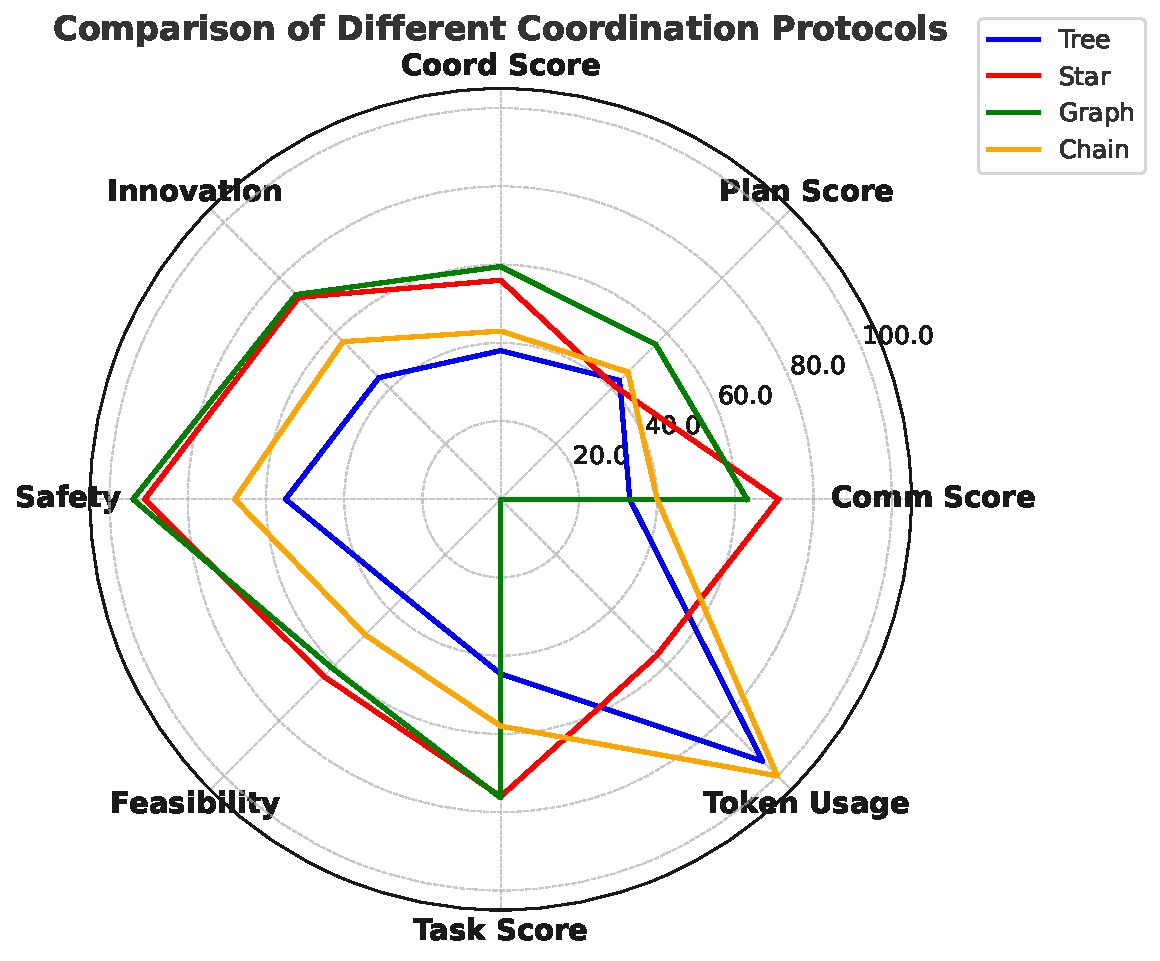
\includegraphics[width=\linewidth]{graphs/comparison_of_coordination_protocols.pdf}
    \caption{Comparison of Different Coordination Protocols.—Tree, Star, Graph, and Chain—across multiple evaluation metrics. Specially, the token usages are scaled such that the lowest value is $0$ and the hightest value is $100$. Details about metrics used for research task can be found at \ref{research_task_metric}}
    \label{fig:coordination_protocol_comparison}
\end{figure}






\begin{figure}[htbp]
    \centering
    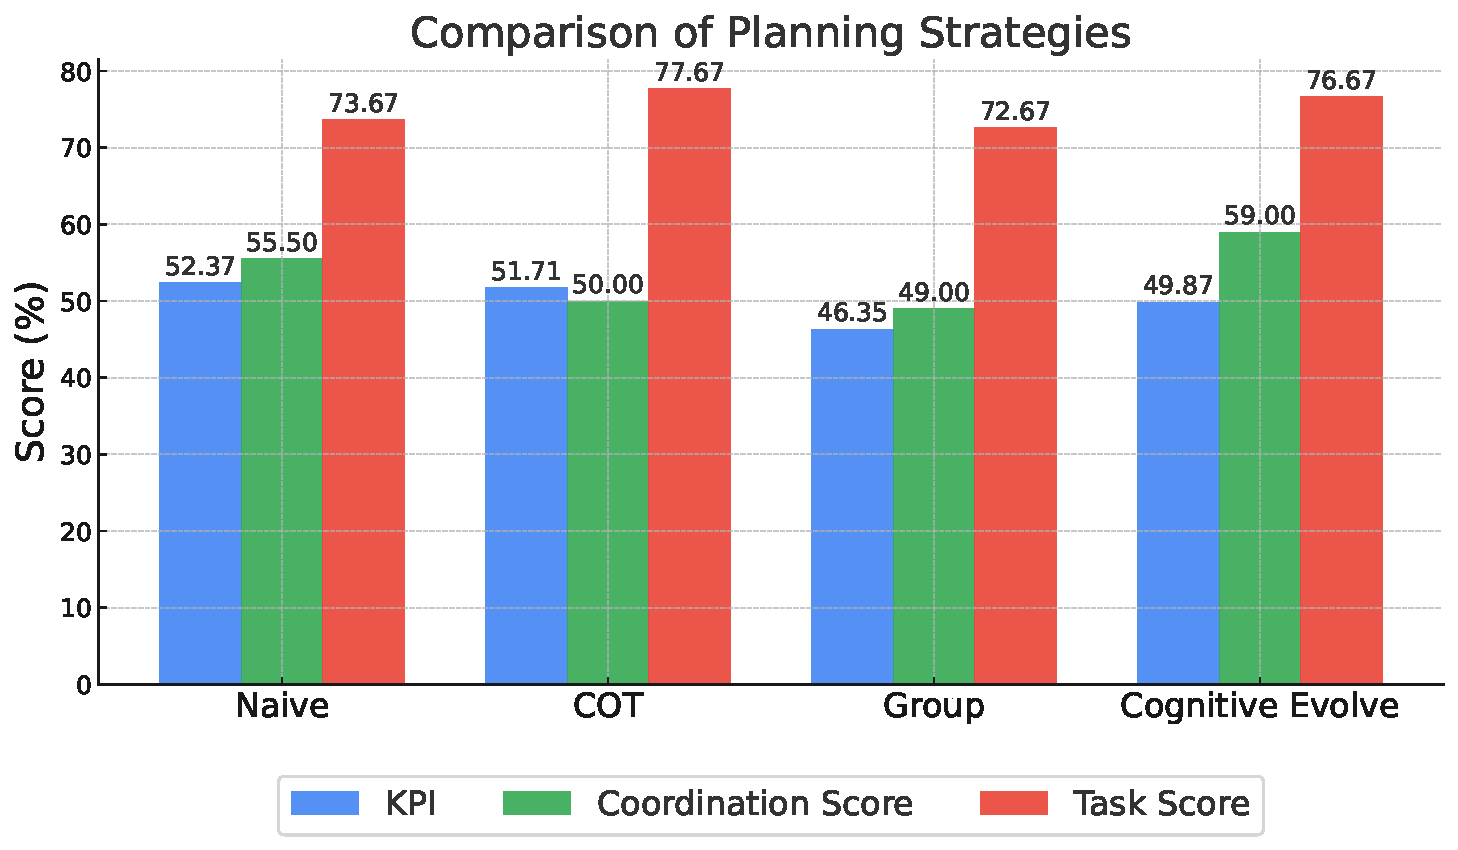
\includegraphics[width=\linewidth]{graphs/research_metrics_legend.pdf}
    \caption{Average Metrics for Research Tasks for different planning prompt strategies. Cognitive Evolve Planning show best result in CS.}
    \label{fig:research_metrics}
\end{figure}

% The \textbf{Cognitive Planning} strategy attains the highest Planning Score (\textbf{4.64}), indicating superior planning abilities. However, the \textbf{Group Discussion} strategy achieves the highest Task Score (\textbf{4.26}), suggesting that collective deliberation among agents enhances task performance.

% The interplay between coordination protocols and planning strategies underscores the importance of selecting appropriate frameworks based on the specific requirements of a task. For instance, tasks that demand high levels of coordination and strategic planning may benefit from centralized protocols like Star coupled with Cognitive Planning strategies. In contrast, tasks prioritizing efficiency and focused execution might be better served by hierarchical protocols like Tree alongside Group Discussion strategies.

\section{Ablation Study}

The goal of our ablation study is to identify the key modules and parameters that affect performance.

\paragraph{Ablation on Different Max Iteration Settings} We evaluate 10 tasks from the Minecraft scenario using six distinct maximum iteration settings. As shown in Fig.~\ref{fig:gpt4o_minecraft_scores}, both task and coordination scores increase from 1 to 7 iterations, but then drop sharply at 10 iterations. At 20 iterations, while the task score shows a recovery, the coordination score remains nearly unchanged beyond 7 iterations. This pattern suggests that, for highly challenging tasks, excessive iterations may lead to coordination degradation—possibly due to communication overhead or conflicting directives emerging over prolonged interactions. These findings underscore the need for adaptive iteration strategies that balance task execution with effective coordination.


\begin{figure}[htbp]
    \centering
    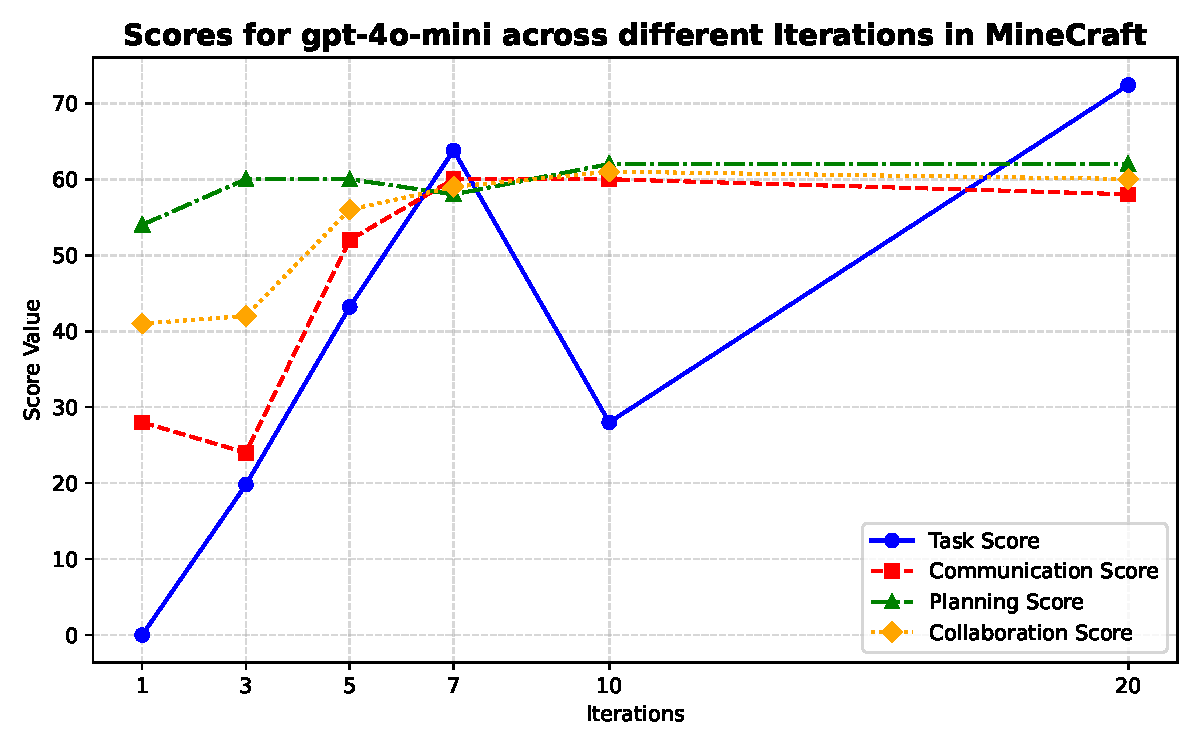
\includegraphics[width=\linewidth]{graphs/scaling_iterations.pdf}
    \caption{Scores for \texttt{gpt-4o-mini} across different iterations in Minecraft. The figure presents Task Score (TS), Communication Score (CS), Planning Score (PS), and Collaboration Score (CoS) over multiple iterations.}
    \label{fig:gpt4o_minecraft_scores}
\end{figure}

\paragraph{Ablation on Different Agent Numbers} We assess configurations with 1, 3, 5, and 7 agents in the research scenario, selecting 20 papers that have at least 7 main authors. As illustrated in Fig.~\ref{fig:scaling_agents}, increasing the number of agents leads to a decrease in the overall KPI, which aligns with the anticipated trade-off between increased collaborative complexity and performance. Notably, the average coordination score improves significantly when moving from 1 to 3 agents, while the average task score increases more gradually. This indicates that a moderate expansion in team size can enhance coordination efficiency, although further increases may introduce additional coordination challenges that counterbalance task performance gains.

\begin{figure}[htbp]
    \centering
    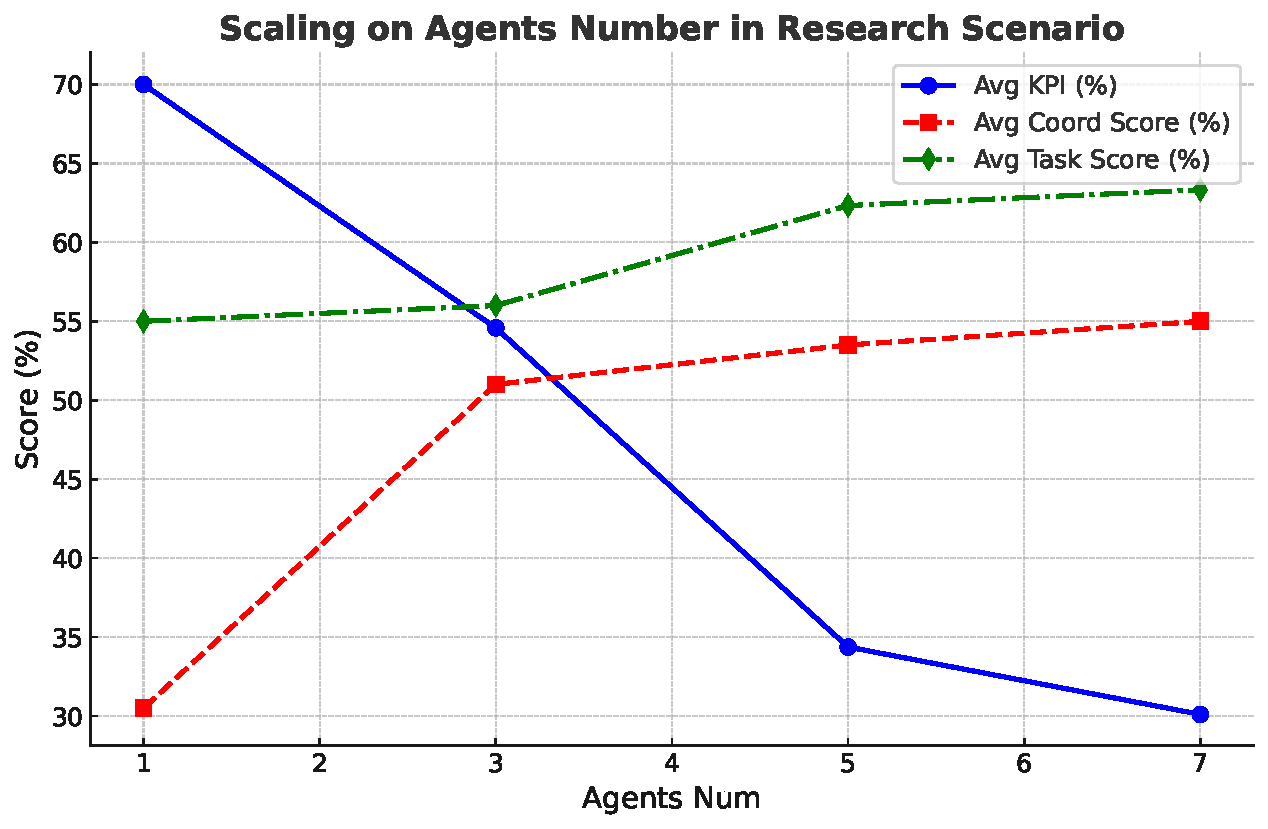
\includegraphics[width=\linewidth]{graphs/scaling_agents_research_scenario.pdf}
    \caption{Scaling on Agents Number in Research Scenario. This figure shows the impact of agent number on KPI, Coordination Score, and Task Score.}
    \label{fig:scaling_agents}
\end{figure}

\section{Emergent Behaviors Analysis}
\label{sec:emergent_behaviors}
In MultiagentBench, goal-driven emergent behaviors are pivotal to team coordination—we argue that these “aha-moments” not only mark when individual agents align their actions toward shared objectives but also catalyze spontaneous multiagent dynamics, unveiling novel coordination strategies and adaptive collective intelligence. (see Appendix~\ref{sec:detailed-results-case-study}). Under information asymmetry and role conflicts, agents display three key patterns (refer to \ref{appendix:case2} and \ref{sec:case_llama33_gpt4o} for Werewolf scenarios, and Section~\ref{fig:negotiation-summary} for Bargaining):

\paragraph{\textbf{Strategic Information Sharing}} Agents selectively disclose key information (e.g., the Seer withholding inspection results) based on trust and context, echoing the "strategic silence" seen in human interactions~\citep{Park2023}. For instance, in \ref{appendix:case2}, both the Seer and Witch (\texttt{gpt-4o}) were overly cautious, missing optimal sharing opportunities and leading to failure. Another case is shown in Fig~\ref{fig:bad_comm_case_1}, where two research agents strategically evolve the research proposal details, combining the strengths of both background knowledge.

\paragraph{\textbf{Trust-Polarized Collaboration}} Role identities drive collaboration splits: over-suspicious villagers may turn against their own, while werewolves can create a "false consensus" through deception~\citep{Fehr2000} and internal execution~\citep{Woolley2010}. As shown in \ref{appendix:case2}, villagers’ excessive caution allowed werewolves to exploit confusion; similar internal friction is evident in Bargaining (\ref{fig:negotiation-summary}).

\paragraph{\textbf{Role-Driven Strategy Iteration}} Throughout the game, roles such as the Seer and Witch adjust their strategies. The Seer, for example, shifts from a conservative to a leadership role (see \ref{sec:case_llama33_gpt4o}), while the Witch moves from hoarding to taking risks. These shifts support the notion that task objectives drive decision-making, aligning with the \textit{AutoGen} framework findings~\citep{Wu2023}.


